\documentclass[Orbiter User Manual.tex]{subfiles}
\begin{document}

\section{Orbital mechanics primer}
\label{sec:orb_mech}
Knowing the underlying physics may not be required to fly a spacecraft (after all, you can drive a car without in-depth knowledge of internal combustion - or electromagnetic induction, depending on when you are reading this), but understanding the laws governing the movement of your craft should provide some additional intellectual satisfaction, or (if that doesn't appeal), may even one day help you get out of an unexpected emergency situation.

\subsection{Kepler's laws of planetary motion}
Johannes Kepler published his three laws of planetary motion in his books \textit{Astronomica Nova} (1609), and \textit{Harmonica Mundi} (1619), refining the Copernican heliocentric model by dropping the assumption of circular orbits, thereby reconciling the theory with observational data.\\
\\
\textbf{Kepler's first law:} A planet orbits the Sun in an ellipse, with the Sun at one of the foci.\\
\textbf{Kepler's second law:} A straight line from the Sun to the planet sweeps out equal areas in equal time intervals.\\
\textbf{Kepler's third law:} The ratio of the square of a planet's orbital period with the cube of its semi-major axis is the same for all planets orbiting the Sun.

\subsection{Elliptic orbits}
An ellipse is a special case of a conic section (the intersection of the surface of a cone with a plane). The equation of a conic section with the origin in one focus (F) is given in polar coordinates (\textit{r}, \textit{v}) by

\begin{figure}[H]
	\centering
	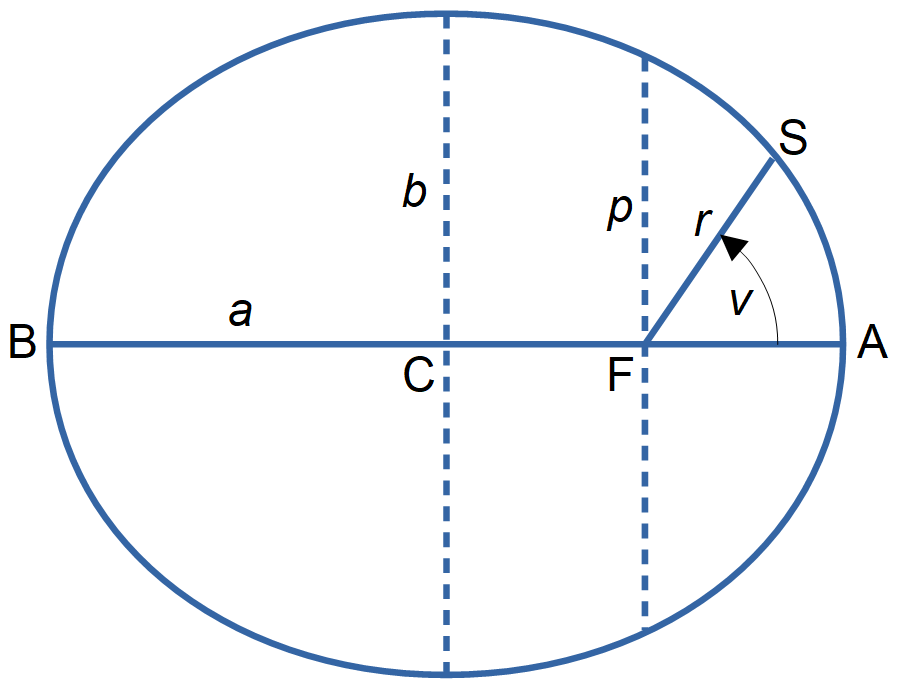
\includegraphics[width=0.5\hsize]{elliptic_orbit.png}
\end{figure}

\[ r = \frac{p}{1 + e \cos v} \]

\noindent
with parameters \textit{e} (eccentricity) and \textit{p} (semi-latus rectum). An ellipse is characterised by eccentricity 0 $\leq$ \textit{e} < 1 (where a circle, e = 0, is taken as the bounding case for an ellipse). The shape of the ellipse is commonly defined by the two parameters \textit{e} and \textit{a} (semi-major axis, the longest semi-diameter), given by

\[ a = \frac{p}{1 - e^{2}} \]

\noindent
Secondary shape parameters can be derived, including the semi-minor axis (shortest semi-diameter) \textit{b}

\[ b = \frac{p}{\sqrt{1 - e^{2}}} = a \sqrt{1 - e^{2}} \]

\noindent
periapsis distance FA (where periapsis A is the point on the ellipse closest to the focus)

\[ r_{pe} = r(v=0) = \frac{p}{1 + e} = (1 - e) a \]

\noindent
and apoapsis distance FB (where apoapsis B is the point on the ellipse farthest from the focus)

\[ r_{ap} = r(v=\pi) = \frac{p}{1 - e} = (1 + e) a \]

\noindent
Kepler's laws successfully described the motion of celestial bodies in accordance with the observations, but they didn't provide a reason (the underlying forces) for this motion. This was provided a few decades later by Isaac Newton.

\subsection{Newton's laws of motion}
Newtonian mechanics provides the general framework for describing the motion not only of celestial bodies, but all objects according to their mass (including falling apples). More than three centuries later, Newtonian dynamics is still an appropriate tool for describing the dynamics of a system of bodies for most practical situations (such as those encountered in Orbiter), where the difference to predictions from general relativity (today's accepted best theory at large scales) are negligible.\\
\\
\textbf{Newton's first law (law of inertia):} An object on which no external force is acting remains at rest or continues moving at a constant velocity.\\
\textbf{Newton's second law:} An object experiences an acceleration that is proportional (and in the same direction) as the sum of all forces acting on it, and inversely proportional to its mass.

\[ \textbf{a} = \frac{1}{m} \sum_{i} \textbf{F}_{i} \]

\noindent
\textbf{Newton's third law:} For every action (force of an object 1 on another object 2) there is an equal and opposite reaction from 2 on 1:

\[ \textbf{F}_{21} = - \textbf{F}_{12} \]

\subsection{Newton's law of gravitation}
Newton introduced the notion of a universal attractive force that works between any two objects. The magnitude of this force is proportional to the object masses $m_{1}$ and $m_{2}$, and inversely proportional to the square of their distance $r_{12}$:

\[ F_{12} = G \frac{m_{1}m_{2}}{r_{12}^{2}} \]

\noindent
where proportionality factor \textit{G} is the \textit{universal gravitational constant}. The direction of the forces is along the straight line from one object to the other:

\[ \textbf{F}_{12} = \hat{\textbf{r}}_{12} F_{12}, \quad \textbf{F}_{21} = - \hat{\textbf{r}}_{12} F_{12} \]

\noindent
where $\hat{\textbf{r}}_{12}$ is the unit vector pointing from object 1 to 2.\\
It is possible to derive Kepler's laws from Newton's laws of motion and gravity. This derivation can be found in most textbooks on astrophysics. It requires some calculus (which was developed by Newton for exactly this purpose, in parallel with the work of Gottfried Leibniz). Expressing Kepler's laws in terms of Newtonian dynamics leads to some useful orbital parameters:\\
The orbital period of an object orbiting a body with mass M is given by

\[ T = \frac{2 \pi}{\sqrt{\mu}} \sqrt{a^{3}} \]

\noindent
with \textit{standard gravitational parameter} $\mu = GM$.\\
The orbital speed \textit{v} as a function of radius \textit{r} is

\[ v = \sqrt{\mu \left(\frac{2}{r} - \frac{1}{a}\right)} \]

\noindent
Maximum and minimum speed occur at periapsis and apoapsis, respectively:

\[ v_{pe} = \sqrt{\frac{(1 + e) \mu}{(1 - e) a}}, \quad v_{ap} = \sqrt{\frac{(1 - e) \mu}{(1 + e) a}} \]

\noindent
and the mean orbital speed is

\[ \bar{v} = \frac{2 \pi a}{T} = \sqrt{\frac{\mu}{a}} = n a \]

\noindent
with \textit{mean angular motion} $n = 2 \pi / T$.\\
The \textit{specific orbital energy} (or vis-viva energy) \textit{E} is the sum of potential energy $E_{p}$ and kinetic energy $E_{k}$ of an orbiting body. \textit{E} is constant along the orbit.

\[ E = E_{k} + E_{p} = \frac{v^{2}}{2} - \frac{\mu}{r} = - \frac{1}{2} \frac{\mu^{2}}{h^{2}}(1 - e^{2}) \]

\noindent
where \textit{h} is the specific angular momentum of the orbiting body. For specific types of orbit, \textit{E} is given by

\[ E =
\left\{
\begin{array}{ll}
	-\frac{\mu}{2a} & e < 1 \\
	0 & e = 1 \\
	\frac{\mu}{2a} & e > 1 \\
\end{array} 
\right. \]

\subsection{Orbital elements}
The orbit of an object around a central body is completely defined by a set of 6 scalar parameters. In addition to the two parameters \textit{a} and \textit{e} discussed above that describe the shape of the ellipse, a further parameter $\omega$ (argument of periapsis) defines the rotation angle of the ellipse in the orbital plane. Two parameters \textit{i} (inclination) and $\Omega$ (longitude of the ascending node) define the orientation of the orbital plane in space relative to a reference coordinate system (e.g. plane of the ecliptic with vernal point {\Aries} as reference direction), and a final parameter \textit{v(t)} (true anomaly) at epoch defines the angular position of the orbiting object along the orbit at a specific time \textit{t}. These are the Keplerian or 2-body elements of an unperturbed orbit. Equivalently, the orbit can also be defined by the \textit{state vectors} of the orbiting object at a given time: position \textbf{r}(t) and velocity \textbf{v}(t). It is possible to calculate the orbital elements from the state vectors and vice versa.

\begin{figure}[H]
	\centering
	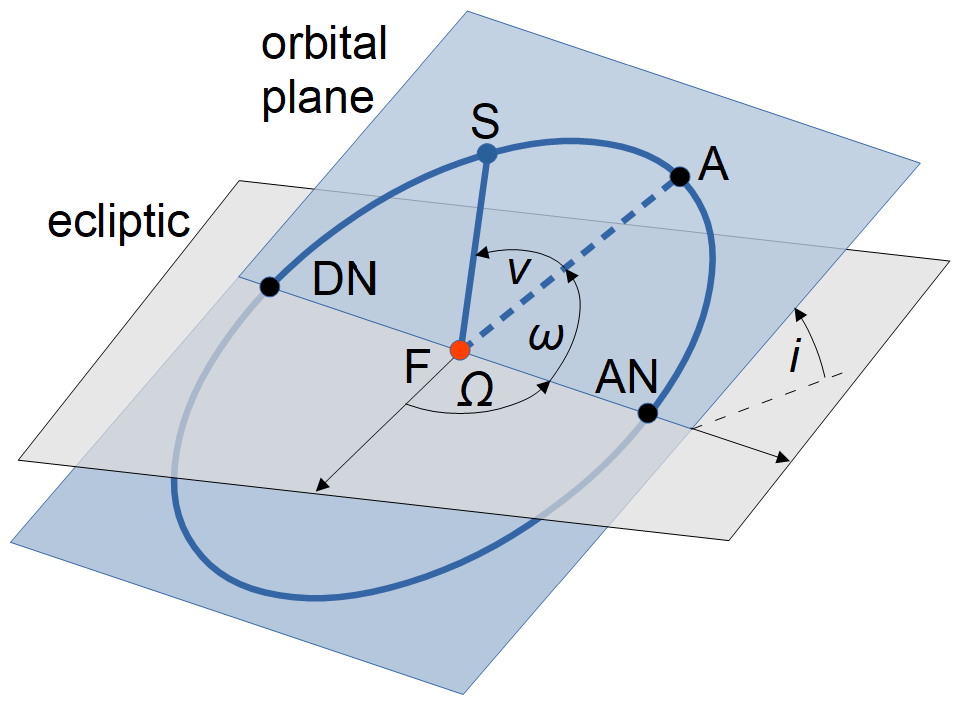
\includegraphics[width=0.5\hsize]{orbital_elements.png}
\end{figure}

\noindent
From Newtonian dynamics we know that Kepler's laws strictly apply only to two-body problems. In the solar system containing multiple bodies which all exert a gravitational force on each other, all orbits are perturbed to some extent from the elliptical shape. In some cases these perturbations are small, but often they cannot be neglected. For example, the Earth's orbit around the Sun is significantly affected by the gravitational influence of its relatively large moon. In this case, it is more appropriate to describe the trajectory the \textit{barycentre} (the centre of mass) of the Earth-Moon system around the Sun as a two-body problem, and the orbits of Earth and Moon around each other as a separate two-body problem on top of it. If even more precision is required, e.g. to factor in the gravitational influence of other planets, an n-body treatment is required, which can generally only be solved numerically.\\
In perturbed orbits, the orbital elements change over time. Computing the 2-body elements from the state vectors at a specific time $t_{0}$ results in the expression of an orbit that the orbiting object would follow in the absence of perturbing influences (osculating orbit). The elements are the \textit{osculating elements} at $t_{0}$.

\subsection{Kepler's equation}
Computing the true anomaly \textit{v} is not trivial for eccentric orbits, because the orbital velocity is changing along the orbit according to Kepler's second law. It is sometimes useful to substitute \textit{v} with the \textit{mean anomaly M}, a parameter that is changing linearly with time:

\[ M(t) = n(t - t_{0}) \]

\noindent
where $t_{0}$ is the time of periapsis passage. M is the angular position of a body in a circular orbit with the same semi-major axis \textit{a} (and thus the same orbital period \textit{T}) and the same periapsis passage time $t_{0}$.

\begin{figure}[H]
	\centering
	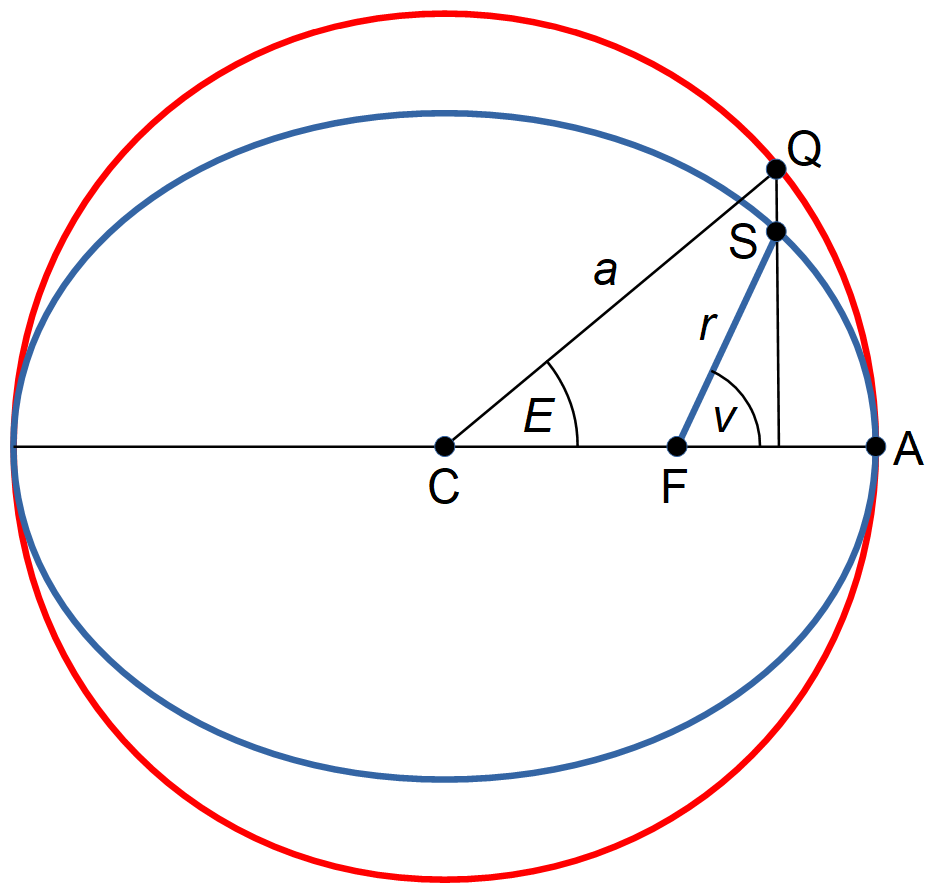
\includegraphics[width=0.5\hsize]{mean_anomaly.png}
\end{figure}

\noindent
To compute true anomaly from mean anomaly, we first introduce the \textit{eccentric anomaly E}: Define a circle with radius \textit{a} whose centre coincides with the centre of the elliptic orbit. Project the object position S perpendicular to the semi-major axis onto the circle (Q). Then \textit{E} is defined as the angle ACQ between periapsis A and Q, measured at the centre C of the circle.\\
The relationship between orbit radius \textit{r} and \textit{E} is given by

\[ r = a (1 - e \cos E) \]

\noindent
\textit{v} can be computed from \textit{E} by

\[ \tan \frac{v}{2} = \sqrt{\frac{1 + e}{1 - e}} \tan \frac{E}{2} \]

\noindent
and \textit{E} is related to \textit{M} via Kepler's equation

\[ E(t) - e \sin E(t) = M(t) \]

\noindent
which cannot be solved in closed form, but generally requires an iterative solution.

\subsection{Sphere of influence and patched conic approximation}
Planning the trajectory of an interplanetary space probe requires the solution of a multi-body problem that takes into account the gravitational influence of Earth, the Sun and the target planet(s) and possibly their moons. This usually involves a numerical simulation that propagates the flight path in time, given a set of initial conditions and potential mid-flight manoeuvres. Such a solution can be computationally expensive, in particular if many trajectory simulations are required, for example to find suitable launch parameters for a trip that involves multiple planet encounters and gravity assist manoeuvres.

\begin{figure}[H]
	\centering
	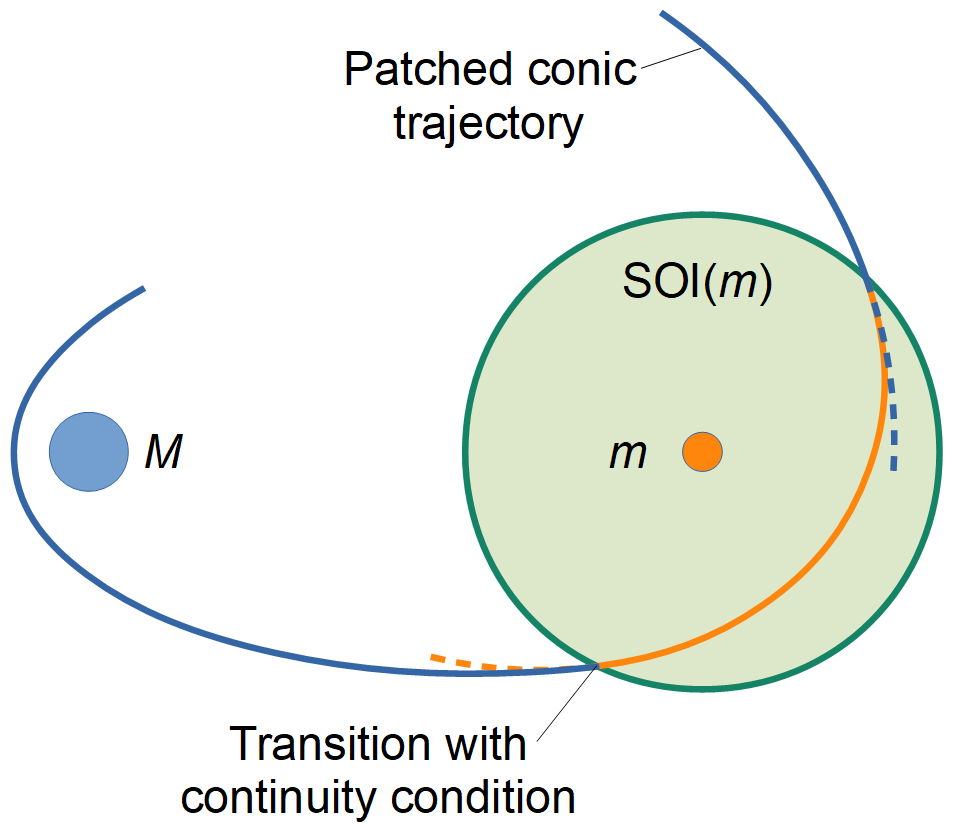
\includegraphics[width=0.5\hsize]{soi.png}
\end{figure}

\noindent
An alternative to the full multi-body solution is the \textit{patched conic approximation}. Given two gravitational sources with masses \textit{M} and \textit{m}, the less massive body \textit{m} is assigned a \textit{sphere of influence}, in the simplest form defined as a sphere with radius

\[ r_{SOI} = a \left( \frac{m}{M} \right)^{2/5} \]

\noindent
where \textit{a} is the semi-major axis of the orbit of \textit{m} around \textit{M}. The region of influence of \textit{M} is all space outside the smaller body's SOI.\\
The spacecraft on a point along its trajectory is assumed to be under the gravitational influence of only the single body whose SOI is currently traversed. As soon as the SOI boundary of another body is crossed, that body's gravitational field is exclusively used for the computation of the next part of the trajectory, subject to the boundary condition that the state vectors (position \textbf{r} and velocity \textbf{v}) are continuous across the SOI boundary.\\
In the solar system, SOI can be assigned for each planet or other body orbiting the Sun. On a second level, a planet's moons may be assigned their own SOI that are embedded in the planet's SOI.\\
The patched conic method is not exact - in particular at the SOI boundaries, where the gravitational influences of the two bodies are approximately equal, neglecting one of them may lead to errors in the trajectory prediction. However, it can be a reasonable initial estimate for designing a mission, and can be refined by a precise numerical multi-body simulation if required.

\end{document}
